\section{Case 2: Kompromitterte brukerkontoer ved NTNU}


\subsection{Problemforståelse}

\subsubsection{Kritiske hendelser}
Sammen med oppgavebeskrivelsen fikk vi en liste over loggførte sikkerhetshendelser som hadde foregått det siste året hvor kompromitterte kontoer var involvert. Dataene ble sortert i synkende rekkefølge og lagt inn i en tabell for å visualisere frekvensen til de enkelte sikkerhetshendelsene, og dermed fokusområdene til trusselaktørene. 

\begin{table} [H]
    \begin{tabular}{ | m{18em} | m{18em} | }
        \hline
            \cellcolor{yellow} Sikkerhetshendelser & \cellcolor{yellow} Frekvens \\
        \hline
            Spam & 46  \\
        \hline
            Misuse (uthenting av forskningsartikler) & 26 \\
        \hline
            Negligible/Fixed/Failed Attack  & 8 \\
        \hline
            Phishing & 7 \\
        \hline
            Whaling & 2 \\
        \hline
            Brute force & 2 \\
        \hline
            DDOS out & 1 \\
        \hline
            Traded credentials & 1 \\
        \hline
            Hackingtools exploits and kits & 1 \\
        \hline
            Copyright/Piracy & 1 \\
        \hline
    \end{tabular}
    \caption{Oversikt over hva kompromitterte ansattkontoer blir brukt til}
    \label{kritisk_tabell_2}
\end{table}

Fra tabellen ser vi at spam er den hendelsen med høyest frekvens, men etter diskusjon med oppdragsgiver var ikke dette problemet av størst viktighet. Det er fordi dette er noe som enkelt blir lagt merke til og er trolig ikke hovedgrunnen til at aktørene aktivt går inn for å kompromittere NTNU sine brukerkontoer. Når det kommer til misuse i tabellen ovenfor referer det til hendelser der uvedkommende misbruker NTNU sine ressurser, spesielt i form av å stjele forskningsartikler på NTNU sin regning. Dette var en av de største problemene med kompromittering av kontoene, siden det førte til økonomisk tap for NTNU og fare for utestengelse fra artikkeldatabasene. 

\subsection{Idémyldring}
I denne fasen ble det gjort en idémyldring. Problemet som ble fremhevet var hvordan brukerkontoer ble kompromittert. Resultatet fra idémyldringen, gruppert i henhold til likhetstrekk, vises i figur \ref{fig:case2-idemyldring} under. 

\begin{figure}[H]
    \centering
    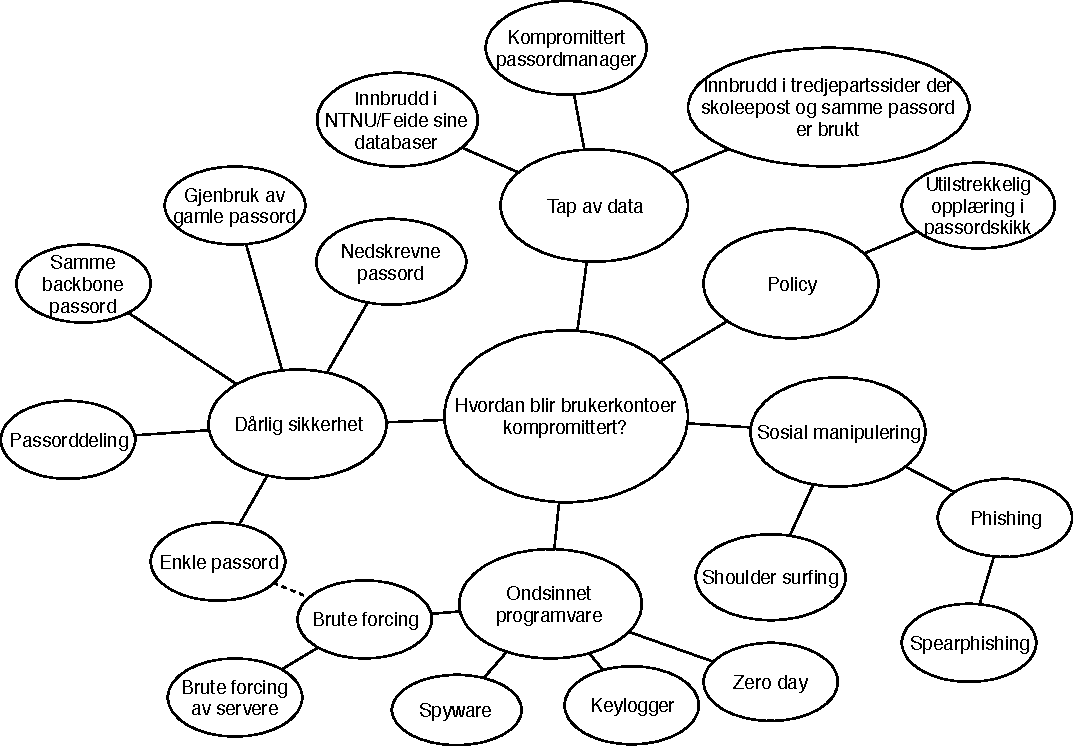
\includegraphics[scale=0.5]{case_2/bilder/idemyldring.pdf}
    \caption[Idémyldring]{Resultater og gruppering av idémyldringen}
    \label{fig:case2-idemyldring}
\end{figure}

Resultatene er gruppert inn i 4 hovedkategorier:
\begin{description}
    \item [Dårlig sikkerhet] er alt fra enkle passord til passordgjenbruk.
    \item [Tap av data] inkluderer at for eksempel sider som dropbox har en lekkasje av brukere.
    \item [Sosial manipulering] vil si å få tak i informasjon ved å lure noen.
    \item [Ondsinnet programvare] er programvare brukt som hjelpemiddel for å få tak i brukerinformasjon.
\end{description}

\subsection{Datainnsamling}
Under idémyldringen ble det avdekket en rekke faktorer som kunne være medvirkende i at ansatte og studenter ved NTNU fikk sin konto på avveie. Vi brukte denne informasjonen aktivt da spørreundersøkelsen ble konstruert. Spørreundersøkelsen slik den fremstår for respondenten finnes i vedlegg \ref{undersokelse_norsk}. Når spørsmålene ble laget ble det bestemt hypoteser til spørsmålene. Disse er listet i tabell \ref{tab:case2-hypoteser} under. 

% Table generated by Excel2LaTeX from sheet 'Ark2'
\begin{table}[H]
  \centering
  \caption{Hypoteser til spørsmålene}
    \begin{tabular}{|p{20.215em}|p{20.57em}|}
    \hline
    \rowcolor{yellow} Spørsmål & Hypoteser \\
    \hline
    Din alder? & Eldre er overrepresentert i statistikken over tapte kontoer \\
    \hline
    Ditt kjønn? & Flere kvinner enn menn har blitt kompromittert \\
    \hline
    Hva er din primærrolle ved NTNU? & Det er ansatte som er målgruppen til trusselaktørene \\
    \hline
    I hvilken by jobber/studerer du primært? & Gjøvik har høyere sikkerhetskompetanse \\
    \hline
    I hvor mange år har du jobbet/studert ved NTNU eller de tidligere høgskolene? & Folk med lavere ansiennitet kjenner universitetets retningslinjer bedre \\
    \hline
    Når fant du ut at NTNU kontoen din var blitt kompromittert? & Folk vet ikke at de har blitt kompromittert før de blir kontaktet \\
    \hline
    Har du noen formening om hvor lang tid kontoen var kompromittert før Seksjon for Digital Sikkerhet kontaktet deg? & Ingen hypotese grunnet vagt spørsmål \\
    \hline
    Har du noen formening om hvordan kontoen din ble kompromittert? & Ingen hypotese grunnet åpent svar \\
    \hline
    Bruker du din NTNU e-post til å registrere deg på ulike tjenester på nett i forbindelse med jobben/studiet? & Over halvparten bruker NTNU e-post til tjenester i forbindelse med jobb \\
    \hline
    Bruker du din NTNU e-post til å registrere deg på tjenester på nett til privat bruk? & Under halvparten bruker NTNU e-post til privat bruk \\
    \hline
    På en skala fra 1-6, der 1 er lite bevisst og 6 er svært bevisst, hvor bevisst er du på sikkerhet når du... & \multirow{4}[2]{*}{Folk er generelt sett lite bevisste} \\
    besøker nettsider? & \multicolumn{1}{r|}{} \\
    lager passord? & \multicolumn{1}{r|}{} \\
    sjekker e-post? & \multicolumn{1}{r|}{} \\
    \hline
    Har du i din tid hos NTNU lagt merke til phishing-forsøk mot deg på din NTNU e-post? & Phishing er en svært utbredt angrepsvektor \\
    \hline
    Har du blitt lurt av phishing på din NTNU e-post? & Av de som har blitt kompromittert har under en tredjedel blitt lurt av phishing \\
    \hline
    Har du i løpet av din tid ved NTNU eller de andre høgskolene, oppdaget virus eller annen skadevare på maskinen din? & Virus og annen skadevare er utbredt \\
    \hline
    Bruker du ditt NTNU passord på flere tjenester? & Passordgjenbruk er utbredt \\
    \hline
    Brukte du regler til å generere ditt NTNU passord? & De fleste bruker ikke passordregler til å generere passord \\
    \hline
    Er ditt NTNU passord tilfeldig sammensatt av bokstaver, tall og/eller tegn? & De fleste bruker ikke tilfeldig sammensatte passord \\
    \hline
    Hvor mange tegn består ditt NTNU passord av? & Over halvparten har passord på under 12 tegn \\
    \hline
    Har du i løpet av din tid ved NTNU delt NTNU passordet ditt med andre? & Passorddeling er ikke særlig utbredt \\
    \hline
    Omtrent hvor ofte bytter du ditt NTNU passord? & Passord byttes for det meste sjeldnere enn hvert andre år \\
    \hline
    Bruker du en passordmanager? & De fleste bruker ikke passordmanager, og mange vet ikke engang hva det er \\
    \hline
    På en skala fra 1 til 6, hvor godt kjent er du med... & \multirow{4}[2]{*}{Det er svært lite kjennskap til retningslinjer} \\
    NTNU sine retningslinjer for behandling av brukernavn, passord og andre autentiseringsdata? & \multicolumn{1}{r|}{} \\
    IT reglementet til NTNU? & \multicolumn{1}{r|}{} \\
    NTNU sine prinsipper for informasjonssikkerhet? & \multicolumn{1}{r|}{} \\
    \hline
    Har du fått opplæring i passordsikkerhet fra NTNU? & Under en fjerdedel har fått opplæring i passordskikk fra NTNU \\
    \hline
    \end{tabular}%
  \label{tab:hypoteser}%
\end{table}%

Av de som e-posten ble sendt ut til fikk vi totalt 72 gyldige respondenter, mens 26 stoppet rett etter åpning av undersøkelsen eller underveis. Undersøkelsen var aktiv i perioden fra 20. April til og med 27. April. I løpet av denne tiden ble det sendt ut én purring den 25. April. 

\subsection{Dataanalyse}


\subsection{Rotårsaksidentifisering}


\subsection{Rotårsakseliminering}


\subsection{Løsningsimplementering}


\subsection{Diskusjon}
